\documentclass[10pt, twocolumn]{article}

\input{template.tex}

\title{Towards a random-based approach for synthetic pandas query generation}

\author{
  Liam Scalzulli \\
  McGill University \\
  \href{mailto:liam.scalzulli@mail.mcgill.ca}{liam.scalzulli@mail.mcgill.ca}
}

\date{\today}

\begin{document}

\maketitle

\begin{abstract}
  This paper presents a random-based procedural algorithm for generating synthetic pandas queries.
  We show that this approach, although vastly simple, can be used to generate valid and complex queries,
  suitable for processes in data science and machine learning, such as evaluating database systems,
  predicting cardinality, and estimating execution times.
\end{abstract}

\section{Introduction}

Query generation workflows remain a critical feature of modern data science and machine learning
workflows. They are involved in cardinality predictor programs, query execution time estimators,
and system performance analyzers.

\spacing
\noindent
Historically, SQL has been the target market for these kinds of programs, leveraging relational
data schemas and existing query sets.

\spacing
\noindent
The widespread adoption of the \textbf{pandas} data analysis library for Python necessitates
further inquiry into how systems might be built to facilitate synthetic query generators for the pandas query language.

\subsection*{What is $pandas$?}

\textbf{pandas} is a data analysis library for Python that provides a fast and efficient DataFrame object for data manipulation with integrated indexing.

\spacing
\noindent
A DataFrame is two-dimensional, size-mutable, potentially heterogeneous tabular data. We can easily create them from native Python structures:

\begin{verbatim}
>>> d = {'col1': [1, 2], 'col2': [3, 4]}
>>> df = pd.DataFrame(data=d)
>>> df
   col1  col2
0     1     3
1     2     4
\end{verbatim}

\noindent
We can write queries against this dataframe (df) using familiar Python syntax.

\spacing
\noindent
Selection ($\sigma$) filters rows based on boolean conditions:

\begin{verbatim}
>>> df[df['col1'] > 1]
   col1  col2
1     2     4
\end{verbatim}

\noindent
Projection ($\pi$) selects specific columns:

\begin{verbatim}
>>> df[['col1']]  # Select only col1
   col1
0     1
1     2
\end{verbatim}

\noindent
Merging ($\bowtie$) combines DataFrames based on common columns:

\begin{verbatim}
>>> df1 = pd.DataFrame({'key': ['A'], 'val1': [1]})
>>> df2 = pd.DataFrame({'key': ['A'], 'val2': [3]})
>>> df1.merge(df2, on='key')
  key  val1  val2
0   A     1     3
\end{verbatim}

\noindent
GroupBy ($\gamma$) operations aggregate data by specified columns:

\begin{verbatim}
>>> df = pd.DataFrame({
...   'group': ['A', 'A', 'B', 'B'],
...   'value': [1, 2, 3, 4]
... })
>>> df.groupby(by=['group']).agg('sum')
       value
group
A          3
B          7
\end{verbatim}

\noindent
These fundamental operations form the basis for more complex queries that can be generated by our algorithm. When combined, they enable sophisticated data manipulation and analysis capabilities.

\subsection*{Prior Art}

Work has been done at McGill University in the Distributed Information Systems Group on a query generator for the \textbf{pandas} query language.

\spacing
\noindent
This generator has taken on a few iterations, and each iteration has tacked on complexity, culminating in
an approach that could benefit from a restructuring.

\spacing
\noindent
Below I will describe these iterations and how they relate to each other:

\spacing
\begin{itemize}
    \item Iteration 1 - \textit{Building a foundation}.

    \spacing
    This first iteration worked on by Dailun Li converted pandas operations into an intermediate
    representation (IR) in Python, e.g. \texttt{df[df[ <conditions>]]} would get translated into \texttt{Selection(df, <conditions>)} [3]. This IR would then get converted into a string, the final query result.

    \spacing
    The IR is flat, which is unable to accommodate any sub-queries within merge operations, and the output is single-line only.

    \spacing
    This iteration generated queries without merges first, calling them 'unmerged' queries, and then combining them later on to form 'merged' queries.
    \spacing

    \item Iteration 2 - \textit{Describing your data}.

    \spacing
    This second iteration worked on by Hongxin Huo invented a schema format (JSON) required as input by the user in order to generate queries [2].

    \spacing
    This schema describes meta-information of the underlying data we're interested in generating queries for. For instance, it includes things such as column names, their types, valid data ranges, foreign key relationships, etc.

    \spacing
    They then generate what are called 'base' queries, which are queries that are composed solely of selection and projection operations.

    \spacing
    For each of these 'base' queries, more selections and projections are tacked onto them. They then try to merge these queries together, forming 'merged' queries. This is a slight modification of the approach adopted by the first iteration.

    \spacing
    This iteration also adopts tree-based structures, allowing for sub-queries within merge operations, with support for multi-line output.
    \spacing

    \item Iteration 3 - \textit{User-input driven generation}.

    \spacing
     The third iteration worked on by Ege Satir extended the program with more custom user input
     to drive the query generation process [1], in addition to adding support
     for more data types in the required schema format. It also adds a better selection generation algorithm than was previously devised.
\end{itemize}

\noindent
This iteration is focused on consolidating this approach into a single, unified random-based algorithm where we start with two user inputs: a schema describing the underlying data we're generating queries for, and parameters that describe information about a single generated query. It is inspired by ideas from all three approaches to achieve its result.

\section{Problem Statement}
The generation of synthetic database queries presents several
key challenges that this work aims to address:

\begin{enumerate}
  \item \textbf{Query Validity}: Generated queries must be
    syntactically correct and logically consistent, ensuring
    they can execute successfully against real datasets.

  \item \textbf{Human-like Structure}: The queries should
    reflect patterns commonly used by data analysts, avoiding
    artificial or unrealistic constructions that might bias
    downstream applications.

  \item \textbf{Complexity Control}: The generation process
    should support varying levels of query complexity, from
    simple operations to multi-stage transformations combining
    multiple DataFrame operations.
\end{enumerate}

\noindent
Formally, given a DataFrame schema $S$, parameters that constrain the query generation process $P_{Q}$, and a set of valid
pandas operations $O = \{\sigma, \pi, \bowtie, \gamma\}$, we
aim to generate a query $Q$ such that:

\begin{itemize}
  \item $Q$ is a valid composition of operations from $O$, satisfying the constraints given by $P_{Q}$.
  \item $Q$ produces a non-empty result set when executed on data conforming to schema $S$.
  \item $Q$ exhibits structural similarities to human-written queries in terms of operation frequency and complexity.
\end{itemize}

\noindent
Our solution focuses on a randomized approach that balances
simplicity with effectiveness, while maintaining control over
the statistical properties of the generated queries.

\section{Algorithm}

The algorithm is concerned with solving the query generation problem in the most simple manner. To achieve this we leverage a wide array of user input to guide our generation steps, using random number generators where applicable.

\subsection*{Input}

To start, we accept a schema $S$. This schema gives us meta-data about the data we're generating queries for. It contains information such as the primary keys for tables, foreign key relationships, column information, etc. This information guides us throughout the various sub-algorithms employed for each operation type.

\spacing
\noindent
Moreover, we accept a few parameters that describe the structure of individually generated queries:

\begin{itemize}
  \item Probability of generating a selection ($P_{\sigma}$).
  \item Maximum number of selection conditions ($C_{\sigma}$).

  \spacing
  These two inputs are used when generating selections for each query. The probability that a query generates a selection is denoted by $P_{\sigma}$. If we're generating a selection, we then use $C_{\sigma}$ to determine how many conditions it has by choosing a random number between 1 and $C_{\sigma}$.
  \spacing

  \item Probability of generating a projection ($P_{\pi}$).
  \item Maximum number of projection columns ($C_{\pi}$).

  \spacing
  Similar to selections, we use $P_{\pi}$ to determine if we're generating a projection for a query. If we do, we use $C_{\pi}$ to determine how many columns it has by choosing a random number between 1 and $C_{\pi}$. The number of columns we project will always be between 1 and $C_{\pi}$.
  \spacing

  \item Maximum number of merge operations ($N_{\bowtie}$).

  \spacing
  This input determines the maximum amount of merges a query can have. We choose the number of merges for a query by generating a random number between 0 and $N_{\bowtie}$.
  \spacing

  \item Probability of generating a group-by ($P_{\gamma}$).
  \item Maximum number of group-by columns ($C_{\gamma}$).
  \item Maximum number of aggregation columns ($C_{\Sigma}$).

  \spacing
  Similar to selections and projections, we use $P_{\gamma}$ as the probability that a query will have
  a group-by operation. For pandas-related constraints, we \textit{always} generate a group-by followed by an aggregation
  operation. We choose how many columns to group-by on with $C_{\gamma}$, choosing a random number between 1 and $C_{\gamma}$ and
  what columns to aggregate on using $C_{\Sigma}$, choosing a random number between 1 and $C_{\Sigma}$.
\end{itemize}

\noindent
All this to say, these components inform us what to do during the core query building step of the algorithm.

\subsection*{State}

We maintain a few state variables throughout the algorithm:

\begin{itemize}
  \item Entity ($E$). The acting entity of the query being generated.

  \spacing
  When we generate queries, there's a chance we're going to step recursively to generate a sub-query.
  We need to keep track of the entity we're currently dealing with in order to (1) keep track of which properties we have access
  to given by schema $S$, and (2) use this entity when generating the string representation of the query.
  \spacing

  \item The currently available columns ($C$).

  \spacing
  We need to keep track of what columns we have access to when generating certain operations. If a projection was done beforehand, we don't want to generate a selection using columns outside of that previous projection set.
  \spacing

  \item The required columns ($R$). Used when orchestrating projection operations.

  \spacing
  When we generate a merge, we need to preserve the join key for sub-queries. If we step recursively to generate a sub-query, we
  need to know what columns we must take into account when generating a projection. If we throw away a join column, the entire merge is no longer valid, thus rendering the entire query invalid.
  \spacing

  \item Merge entities ($M$). A set of entities that this query is composed of.

  \spacing
  Let an atomic query be a query that acts on a single entity. A generated query is composed of atomic queries. When merging queries together, we need to consider the entity set given by its atomic query set, because we don't want these sets to intersect. For instance, if we have a query that's composed of entities customers and orders, we don't want to merge it with a query that's composed of a single entity, orders.
\end{itemize}

\noindent
By definition, $R \subseteq C$ holds throughout the life-cycle of the algorithm.


\subsection*{Query Building}

The query building step in the algorithm decides which operation we should be generating, based on the input parameters described above.

\spacing
\noindent
The pseudo-code for this procedure is described as follows:

\spacing
\begin{lstlisting}
if |C| > 0 and $C_{\sigma}$ > 0 and rand() < $P_{\sigma}$
  generate a selection

if |C| > 0 and $C_{\pi}$ > 0 and rand() < $P_{\pi}$
  generate a projection

from 0 to rand(0, $N_{\bowtie}$)
  if we can generate a merge, do it
  otherwise give up

if |C| > 0 and $C_{\gamma}$ > 0 and rand() < $P_{\gamma}$
  generate a group by operation
\end{lstlisting}

\spacing
\noindent
This procedure constrains the generated query in a few subtle ways:

\begin{itemize}
  \item Each individually generated query can have \textbf{at most} 1 selection and 1 projection operation. Generated queries can have sub-queries, so the total amount will vary.
  \item A group by operation is always generated at the end, allowing us to tweak query parameters to ensure we only append one at the end of the outer-most query. This will become more apparent once we describe the merge generation process.
\end{itemize}

\noindent
These subtle constraints are in place because we want generated queries to exhibit structural similarities to human-written queries. Without these constraints, we could generate queries with all sorts of bizarre operation patterns, such as a multitude of projections one after the other.

\subsection*{Operation Types}

As seen above, the query building step dispatches to our individual operation generation algorithms. In this section, we describe the algorithm for each operation type. Our working set of operations is assumed to be $\{\sigma, \pi, \bowtie, \gamma\}$.

\subsubsection*{Selection $(\sigma)$}

Selections, alongside merges, are one of the trickier operations to generate.

\spacing
\noindent
A purely random approach to generating conditions could yield nonsensical results, culminating in an empty intersection. For instance, if we're generating conditions for an entity with an integer property $x$, a possible condition set could be $x < 5 \land x > 10$.

\spacing
\noindent
The goal is to generate a condition set that satisfies the constraints imposed by $C_{\sigma}$ and is logically consistent (no empty intersections).

\spacing
\noindent
Assume the data types and the data ranges for each column on all tables are given by schema $S$. We can proceed with a base algorithm:

\spacing
\begin{lstlisting}
set $COND$ to be an empty list

set $X$ to be rand(1, min($C_{\sigma}$, |C|))

from 1 to $X$
  pick a random column $C_{i}$ $\in$ $C$

  set $T_{i}$ to the type of column $C_{i}$
  set $R_{i}$ to be the range of column $C_{i}$

  generate and append a condition that considers $T_{i}$, $R_{i}$ and references $C_{i}$, to $COND$

select on the condition set $COND$
\end{lstlisting}

\spacing
\noindent
Next we describe generating conditions and adding them to $COND$, while maintaining consistency of the entire condition set.

\spacing
\noindent
Consistency conflicts can only be generated when operating on the same value. For instance, a possible solution to this problem would be to cap the number of conditions per column to 1. Since we want to avoid doing this, we have to figure out a way to satisfy the desired number of conditions while maintaining consistency.

\spacing
\noindent
We approach this problem by keeping track of previously generated conditions for columns, and grouping conditions for each column in parentheses, joined by random operations. For example, a valid condition set would look like (x $\textgreater$ 3 $\land$ x $\textless$ 10) $\lor$ (y = 5) $\land$ (z $\geq$ 10 $\lor$ z $\leq$ 40).

\spacing
\noindent
(TODO: Finish this section with a described algorithm)

\subsubsection*{Projection $(\pi)$}

A projection operation simply selects out of our available columns set $C$ a random subset to project. Before we do this however, we subtract the required column set $R$ from the available columns, appending them right before generating the projection:

\spacing
\begin{lstlisting}
set $P$ to $C$ - $R$

if $P$ is empty
  project $C$

set $X$ to rand(1, min($C_{\pi}$ - |R|, len($P$)))

select a subset $P_{S} \subseteq P$, $|P_{S}| = X$

set $C$ to $P_{S}$ + $R$

project $P_{S}$ + $R$
\end{lstlisting}

\subsubsection*{Merge $(\bowtie)$}

Merge operations are special in the sense that they can produce sub-queries. For instance, inspect the following query:

\begin{verbatim}
nation.merge(
  region[(region['R_NAME'] != 'M')],
  left_on='N_REGIONKEY',
  right_on='R_REGIONKEY'
)
\end{verbatim}

\noindent
We merge the entity $nation$ with rows in $region$ whose $R\_NAME$ property is not equal to $M$.

\spacing
\noindent
Assume we can get foreign key relationships from $S$ by an entity $E$ ($S_{FK}[E]$). These are given as tuples ($c_{l}$, $c_{f}$, $\varepsilon$) where $c_{l}$ is the local column on $E$, $c_{f}$ is the foreign column and $\varepsilon$ is the foreign entity (or table) containing $c_{f}$.

\spacing
\noindent
We use all of this information to suggest a recursive approach, which is outlined in the following algorithm:

\spacing
\begin{lstlisting}
set $candidates$ to an empty list

for $c_{l}$, $c_{f}$, $\varepsilon$ from $S_{FK}[E]$
  if $c_{l} \in C$
    add $c_{l}$, $c_{f}$, $\varepsilon$ to $candidates$

if $candidates$ is empty
  give up, we can't perform a merge

choose a $c_{l}$, $c_{f}$, $\varepsilon$ $\in candidates$

set X to be a new empty query on $\varepsilon$

set parameters for $X$
  $P_{\gamma, X}$ = 0 // Ensures we have no groupby
  $N_{\bowtie, X}$ = $N_{\bowtie}$ - # merges for this query
  ... inherit from the current query

build a query $X$ with $R_{X}$ + $\{c_{f}\}$, $C_{X}$ = all columns on $\varepsilon$

set $C$ to the union of $C$ with the columns returned by $X$

set $M$ to the union of $M$ with the merge entities of query $X$

subtract $N_{\bowtie}$ by the number of merges in query $X$

merge the current query with $X$
\end{lstlisting}

\spacing
\noindent
To get a feel for how this algorithm works, lets take a look at the relational algebra tree for the example query shown above:

\spacing
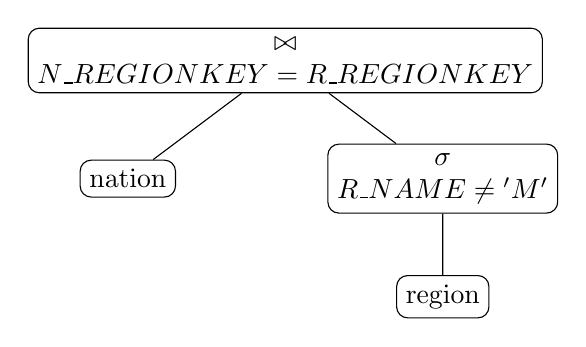
\begin{tikzpicture}[
  level distance=1.5cm,
  level 1/.style={sibling distance=4cm},
  level 2/.style={sibling distance=3cm},
  every node/.style={draw, rounded corners, align=center}
]
\node{$\bowtie$\\$N\_REGIONKEY = R\_REGIONKEY$}
  child {
    node {nation}
  }
  child {
    node {$\sigma$\\$R\_NAME \neq \text{'M'}$}
      child {
        node {region}
      }
  };
\end{tikzpicture}

\spacing
\noindent
Our algorithm starts off with $E = nation$. We hit a merge operation right away, we remember this and start bottom up from a new entity $region$. Once the $region$ query is built we join the two together.

\spacing
\noindent
Lets look at another, more complex, query:

\begin{verbatim}
customer[
  (customer['C_ADDRESS'] != 'm')
].merge(
    nation.merge(
      region[['R_REGIONKEY', 'R_NAME']],
      left_on='N_REGIONKEY',
      right_on='R_REGIONKEY'
    ),
  left_on='C_NATIONKEY',
  right_on='N_NATIONKEY'
).groupby(
  by=['R_REGIONKEY', 'R_NAME']
).agg('count')
\end{verbatim}

\noindent
The relational algebra tree is as follows:

\spacing
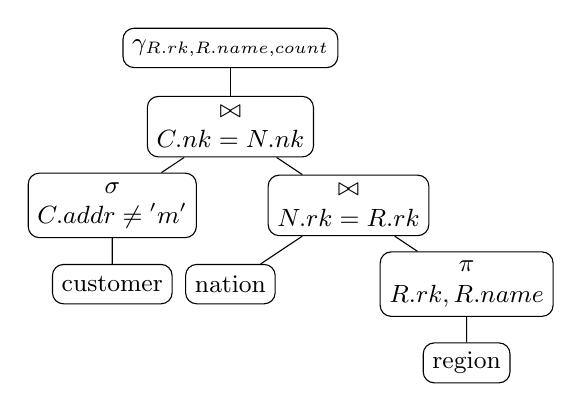
\begin{tikzpicture}[
  level distance=1cm,
  sibling distance=3cm,
  every node/.style={
    draw,
    rounded corners,
    align=center,
    minimum height=0.5cm,
    font=\small
  }
]
\node{$\gamma_{R.rk, R.name, count}$}
  child {
    node{$\bowtie$\\$C.nk = N.nk$}
    child {
      node{$\sigma$\\$C.addr \neq \text{'m'}$}
      child {
        node{customer}
      }
    }
    child {
      node{$\bowtie$\\$N.rk = R.rk$}
      child {
        node{nation}
      }
      child {
        node{$\pi$\\$R.rk, R.name$}
        child {
          node{region}
        }
      }
    }
  };
\end{tikzpicture}

\spacing
\noindent
We start with a left entity $E = customer$. We build this query up until we hit the merge operation, where we then start bottom-up from $nation$, stepping once again recursively building up the $region$ query. We join each atomic query (a specific set of sub-trees) together with merge operations, appending a groupby operation to the outer-most query.

\spacing
\noindent
Queries are \textit{always} built bottom-up starting from individual entities (or tables) described by the schema $S$. Each query has a sole acting entity, and we combine these atomic queries with merge operations to form one large and complex query, which may act on all entities described by $S$.

\spacing
\noindent
We're able sustain such complex recursion trees that maintain query validity simply because we preserve join columns all the way down. The projection generation process always takes into account $R$, a required column set.

\subsubsection*{Groupby $(\gamma)$}

For simplicity, we \textit{always} generate the group-by with an aggregation. Since this is always appended at the end of the outer-most query, we need not worry about required columns, so we pick a random subset from our available columns with a mapping of columns to aggregation functions.

\spacing
\begin{lstlisting}
set X to rand(1, min($C_{\gamma}$, |$C$|))

select a subset $G_{S} \subseteq C$, |$G_{S}$| = X

set $A$ to be C - $G_{S}$

if A is empty
  group by on $G_S$, without aggregation

set Y to be rand(1, min($C_{\Sigma}$, |A|))

select a subset $A_{S} \subseteq A$, |$A_{S}|$ = Y

set $F$ to be an empty mapping

for each column $\in$ $A_{S}$
  map column -> a function, in $F$

group by on $G_S$, aggregate with $F$
\end{lstlisting}

\spacing
\noindent
The mapping of columns to a function should be done knowing the columns type. For instance, a column whose type is string should not get mapped with $mean$. This mapping can be defined statically in code, associating column types with appropriate functions.

\subsection*{Output}

The algorithm outputs a set of operations, call it the resulting operation set $O_{R}$ \text{where} $\forall o \in O_{R}, o \in O$.

\section{Software Implementation}

We provide a full and comprehensive Python package that implements the aforementioned algorithm, called \textbf{pqg}, that lets users generate thousands of complex queries for their schemas very quickly.

\spacing
\noindent
The package contains both command-line and library interfaces, alongside a companion web application with a friendlier user experience.

\begin{figure}[htbp]
  \centering
  \includegraphics[width=0.5\textwidth]{web-view.png}
  \caption{Statistics view in the web application}
\end{figure}

\spacing
\noindent
The core of the tool is written in Python, which consists of the command-line tool and library, whereas the web application is written in React and TypeScript, making use of the library interface distributed over the Python package index (PyPI), using Pyodide.

\spacing
\noindent
The code is fully open source, and it lives at \href{https://github.com/DISLMcGill/pandas-query-generator}{https://github.com/DISLMcGill/pandas-query-generator}.

\subsection*{Results}

The tool is able to generate and execute both single-line and multi-line queries, with options to always ensure they produce some output when ran on sample data. Here are some example queries generated by the tool:

\begin{enumerate}

\item Query with a simple selection, merge and groupby.

\begin{verbatim}
nation[nation['N_NAME'].str.startswith('K')]
  .merge(
    region,
    left_on='N_REGIONKEY',
    right_on='R_REGIONKEY'
  )
  .groupby(by=['R_COMMENT']).agg('count')
\end{verbatim}

\item Multiple merge operations.

\begin{verbatim}
supplier.merge(
  nation.merge(
    region,
      left_on='N_REGIONKEY',
      right_on='R_REGIONKEY'
    ),
    left_on='S_NATIONKEY',
    right_on='N_NATIONKEY'
  )
  .groupby(by=['N_REGIONKEY', 'N_NATIONKEY'])
  .agg('min', numeric_only=True)
\end{verbatim}

\item Multi-line format.

\begin{verbatim}
df1 = lineitem[[
  'L_PARTKEY',
  'QUANTITY',
  'SHIPDATE',
  'RETURNFLAG',
  'SHIPMODE',
  'LINENUMBER'
]]

df2 = partsupp[
  (partsupp['PS_SUPPKEY'] <= 1720)
]

df3 = df2[[
  'AVAILQTY',
  'PS_PARTKEY',
  'PS_SUPPKEY'
]]

df4 = part[[
  'P_NAME',
  'CONTAINER',
  'PT_COMMENT',
  'RETAILPRICE',
  'MFGR',
  'BRAND',
  'SIZE',
  'P_PARTKEY'
]]

df5 = df3.merge(
  df4,
  left_on='PS_PARTKEY',
  right_on='P_PARTKEY'
)

df6 = df1.merge(
  df5,
  left_on='L_PARTKEY',
  right_on='PS_PARTKEY'
)
\end{verbatim}

\end{enumerate}

\noindent
Each of these queries was generated using the \href{https://www.tpc.org/tpch/}{TPC-H} reference schema.

\subsection*{Benchmarks}

Performance was always at the top of mind during implementation, and it shows in the query generation and execution times.

\spacing
\noindent
Below are benchmarks for tasks \textbf{pqg} can handle. We use the \href{https://github.com/sharkdp/hyperfine}{hyperfine} command-line tool to compile an average runtime for these tasks, all ran on an M2 Macbook Pro.

\spacing
\begin{table}[h]
    \centering
    \begin{tabular}{|l|c|}
        \hline
        Task & Time (s) \\
        \hline
        Generating 100 queries & 0.8291 \\
        Generating 1k queries & 1.587  \\
        Producing 1k non-empty result queries & 3.291 \\
        Generating 10k queries & 10.028 \\
        \hline
    \end{tabular}
    \caption{Benchmarks for various tasks}
    \label{tab:benchmarks-table}
\end{table}

\spacing
\noindent
The third iteration provided very few parameters for tweaking the query generation process. It
simply attempted to generate and ensure non-empty results for the number of queries specified. Running hyperfine on the program with parameters equivalent to our \textbf{Producing 1000 non-empty result queries} run gives us \textbf{52.747s} on average.

\spacing
\noindent
Our implementation is \textbf{16.03x}, or \textbf{93.76\%} faster, on average, than the old one.

\subsection*{Next Steps}

There's a ton of cool stuff we can add to this tool, this section describes a few of these ideas:

\begin{enumerate}
  \item Generating logically consistent selection sets.

  \spacing
  We currently adopt a strictly random-based approach when generating selection condition sets. A purely random-based approach could yield nonsensical results, such as sets that contain empty intersections (e.g. $x < 3 \land x > 5$). One possible solution is to only generation 1 condition per column. This should be avoided, however, and the algorithm should support more than one condition per column.
  \spacing

  \item Select aggregation functions based on column types.

  \spacing
  The software currently selects a single aggregation function which gets applied to the rest of the columns which aren't part of the groupby column set. This doesn't make sense in certain cases (e.g. min on a string column). We should take into account column types when generating aggregation functions, and use \textbf{pandas} dictionary syntax when generating these types of operations.
  \spacing

  \item Handle schemas with multiple entities who have the same property names.

  \spacing
  Our generated queries don't disambiguate column names between tables. If a table shares a column name with another, we have no way to tell which table it came from. We should automatically add a unique prefix or suffix when constructing the query output string, so as to allow for duplicate column names in the schema format.
  \spacing

  \item Support multiple output formats.

  \spacing
  We currently only support outputting to a single text file with the command-line interface and web application. We should consider other output formats, such as JSON, Markdown, etc.
  \spacing
\end{enumerate}

\section{Conclusion}

This paper presented a simplified, random-based approach to synthetic pandas query generation. By leveraging user-provided schema information and generation parameters, our algorithm produces complex, valid queries that closely resemble real-world data analysis patterns. The implementation, available as the open-source \textbf{pqg} package, demonstrates significant performance improvements over previous approaches, achieving a 93.76\% reduction in query generation time while maintaining query validity and complexity.

\spacing
\noindent
Key contributions of this work include:
\begin{itemize}
    \item A streamlined algorithm that handles the core pandas operations ($\sigma$, $\pi$, $\bowtie$, $\gamma$) while maintaining query validity through careful state management.
    \item A flexible parameter system that allows fine-grained control over query complexity and structure.
    \item An efficient implementation that can generate thousands of queries in seconds, making it suitable for large-scale testing and analysis workflows.
\end{itemize}

\spacing
\noindent
The success of this approach suggests that complex query generation tasks can be effectively addressed through well-designed random-based algorithms, providing a foundation for future work in automated query generation and testing systems. As pandas continues to evolve as a critical tool in data science workflows, tools like \textbf{pqg} will play an increasingly important role in system evaluation, performance testing, and machine learning applications.

\renewcommand{\refname}{6 \quad References}

\begin{thebibliography}{99}

\bibitem{pandas-satir}
Ege Satir. Customized Query Generation for Pandas. Mcgill University.

\bibitem{pandas-hongxin}
Hongxin Huo. Refined Automated Query Generation for Pandas. Mcgill University.

\bibitem{pandas-dailun}
Dailun Li. Automated Query Generation for Pandas. Mcgill University.

\end{thebibliography}

\end{document}
